\subsubsection{Clarke Transformation and Park Transformation}
The control type chosen for the system is vector control also called field-oriented control and this requires Clarke/Park transformations as well as their inverse counterparts.
The transformations are implemented in the processing system and to limit the amount of calculations needed for each transformation all constants are defined beforehand.

% ******* Clarke Transformation ***********************************
\subsubsection*{Clarke Transform}


The embedded implementation of the Clark transformation as per equation \ref{eq:clarke_transformation} can be seen in code sample \ref{code:clarke}. The function creates two results and therefore instead of returning the values, the variables are declared outside the function calls and a pointer to the variables are parsed into the function.

\begin{lstlisting}[style=c, caption=Embedded Clarke Transformation., label=code:clarke]
/* The Clarke function */
void clarke(f32 *iAlpha, f32 *iBeta, f32 iA, f32 iB, f32 iC){
	*iAlpha = TWO_THIRDS * iA - ONE_THIRD * iB - ONE_THIRD * iC;
	*iBeta  = ONE_OVER_SQRT_THREE * iB - ONE_OVER_SQRT_THREE * iC;
}
\end{lstlisting}

% ************** Park Transformation ***********************************
\subsubsection*{Park Transform}
The embedded implementation of the Park transformation as per equation \ref{eq:park_transformation} can be seen in code sample \ref{code:park}. The transformation involves calculating the sine and cosine of the angle. These two functions are implemented by using look-up tables and are discussed in section \ref{sec:sine_cosine}.

\begin{lstlisting}[style=c, caption=Embedded Park Transformation., label=code:park]
/* The Park function */
void park(f32 *iD, f32 *iQ, f32 iAlpha, f32 iBeta, f32 angle){
	const f32 cosAngle = fastCos(angle);
	const f32 sinAngle = fastSin(angle);
	*iD = cosAngle * iAlpha + sinAngle * iBeta;
	*iQ = -sinAngle * iAlpha + cosAngle * iBeta;
}
\end{lstlisting}

The inverse Clarke and inverse Park transformations can be found in appendix \ref{app:inverse_park} and \ref{app:inverse_clarke}.


\paragraph{Sine and Cosine}
\label{sec:sine_cosine}
The trigonometric functions sine and cosine are implemented with a look-up table to improve performance. The sine function looks up a given angle in the table to find the output of the function. The cosine uses the sine function but offset the angle by $90 ^{\circ}$. 

To limit the amount of memory used only one value is saved per degree which results in $360$ saved values of type \textit{f32} which is based on the type \textit{float}. The variables are $4$ bytes resulting in $1440 bytes \sim 1.5kB$ used.
The maximum error that can exist because of the quantization is the biggest step between two values in the data set. 
The largest error is where the sine/cosine has the largest slope, and this is where it crosses 0 on the y-axis. The error is positive when the slope is positive and negative when the slope is negative. The maximum error is $\pm 1.75 \%$ as can be seen on figure \ref{fig:sinus_lookup_error}. 
\begin{figure}[H]
	\centering
	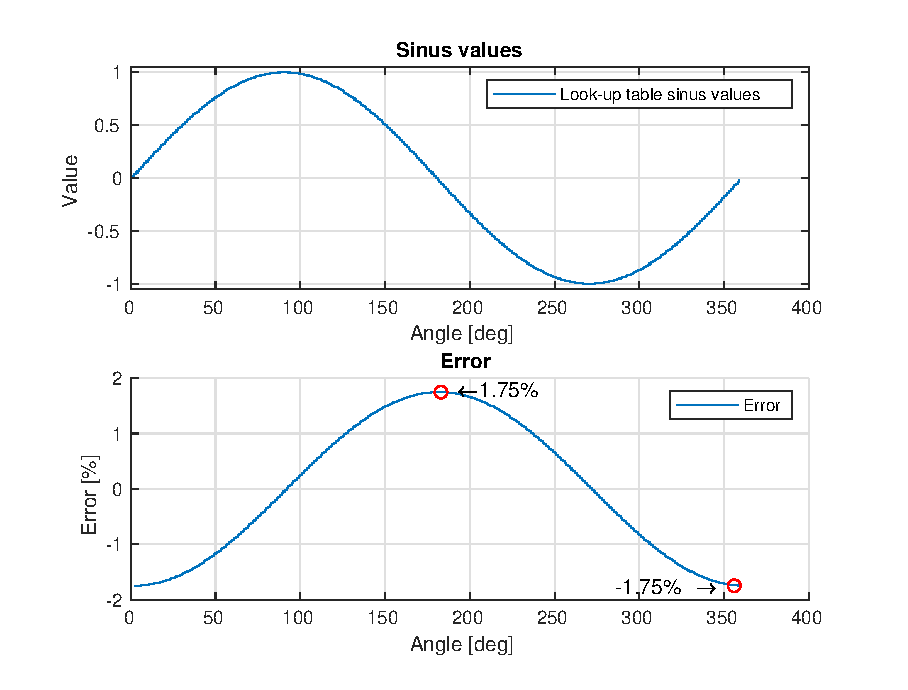
\includegraphics[width=1 \textwidth]{pictures/software/sinus_lookup_error.eps}
	\caption{Error between the real sine value and the look-up table value.}
	\label{fig:sinus_lookup_error}
\end{figure}

The code to perform the sine and cosine can be found in appendix \ref{app:sineCosine}.

% \begin{lstlisting}[style=c, caption=Sine and cosine implemented with look-up tables., label=code:lookup_table]
% /* Sine lookup table */
% #define SIN_N 		360	 // Number of data points in the sine constant array
% const f32 sineValues[] = {0,0.0174524064372835,0.0348994967025010,...};

% /* Function that returns sin(angle) */
% f32 fastSin(f32 angle){
% 	unsigned int index = (unsigned int)angle;       // Truncate decimals
% 	return (f32)sineValues[index % SIN_N];      // 
% }	

% /* Function that returns cos(angle) */
% f32 fastCos(f32 angle){
% 	f32 newAngle = (f32)((int)(angle + 90) % (int)360);
% 	return (f32)fastSin(newAngle);
% }
% \end{lstlisting}